\chapter{LLVM}
\section{History}
The \llvm is a collection of modular and reusable compiler and toolchain technologies to support of static and dynamic Compilation as well as tranparent and lifelong program analysis and transformations of arbitrary programs. \cite{LLVMWebsite, LLVMResearchBeginning}\\
The \llvm former was a reasearch project at the university of Illinois, which was first descripted in a publication in 2004. TODO: Think about sentence
The project was getting so popular that in 2014 the \llvm Foundation was founded for organizing and maintaining the project. \cite{LLVMFoundation}\\
In order to make the \llvm as independent as possible of the programming language used, the \llvmir was created.

\section{Pipeline \cite{IntroLLVM}}
The pipeline of the \llvm (\autoref{fig:llvmPipeline}) translates files containing sourcecode written in an arbitrary programming language into \llvmir, on which the following components operate.
At the end assembler is generated out of the (possibly) newly formed \llvmir by the \generator.
\begin{figure}[!ht]
    \caption{The pipeline of LLVM}
    \label{fig:llvmPipeline}
    \centering
    \begin{tikzpicture}
        \node(languages)[nonLlvmIrNode]{C/C++/Obj-C};
        \node(clang)[nonLlvmIrNode, right=of languages]{clang frontend};
        \node(opt)[llvmIrNode, right=of clang]{\opt};
        \node(generator)[llvmIrNode, below=of opt]{\generator};
        \node(linker)[nonLlvmIrNode, left=of generator]{\linker};
        \path[nonLlvmIrPath] (languages) to (clang);
        \path[llvmIrPath] (clang) to (opt);
        \path[llvmIrPath] (opt) -| ($(opt.north east) + (0.5,0.5)$) -| node[auto]{Pass} (opt);
        \path[llvmIrPath] (opt) to (generator);
        \path[nonLlvmIrPath] (generator) to (linker);
    \end{tikzpicture}
\end{figure}\\
\subsection{clang frontend}\label{subsec:clangfrontend}
More precisly files containing sourcecode are translated by the clang frontend -- currently at least C, C++ and languages based on C are supported -- into \llvmir by adding the option \texttt{-emit-llvm} \enquote{to abstract away from the specifics} \cite{FastScopDetection} of a programming language.
Often also the option \texttt{-S} is passed in order to generate a human readable textfile instead of a \llvmir binary.
\subsection{LLVM Optimizer}\label{subsec:optimizer}
On the received files the \opt can perform steps optimizing and analysing the code.
These steps are called \enquote{Passes}.
They can be explicitly added by specifying appropriate options to the command \texttt{opt} of the \opt.
The option \texttt{-S} can also be specified for the same reasons as in \autoref{subsec:clangfrontend}.\\
It is also possible to add further options by loading multiple libraries using the flag \texttt{-load}.
\subsection{LLVM Code Generator}
When all desired passes are performed the \generator translates the \llvmir into assembler.
\subsection{LLVM Linker}
The \linker finally compiles an executable binary.
\subsection{Control Flow Graph (CFG)}
At any point the current \cfg of a \llvmir file can be visualized:
\begin{figure}[!ht]
    \caption{An example for CFG}
    \label{fig:examplePipeline}
    \begin{minipage}{.7\textwidth}
        \inputminted{c++}{cpp/matmul.cpp}
    \end{minipage}
    \begin{minipage}{.2\textwidth}
        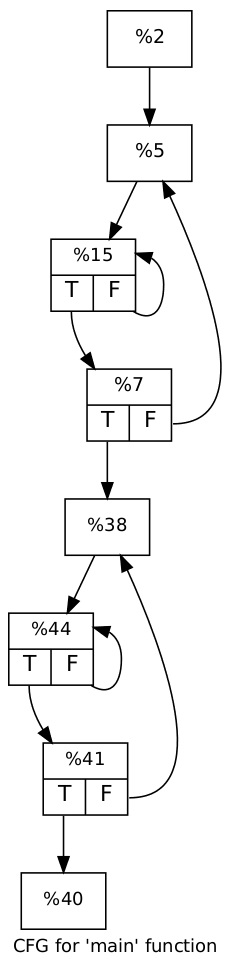
\includegraphics[height=12cm]{gfx/matmulCfg.png}
    \end{minipage}
\end{figure}\\
This can be performed by the following steps/commands:
\begin{enumerate}
    \item Translate the program into \llvmir using the clang frontend.\\
        \texttt{clang -S -emit-llvm matmul.cpp -o matmul.ll}
    \item Show the current \cfg using the \opt.\\
        \texttt{opt -disable-output matmul.ll -view-cfg-only}
\end{enumerate}
